% Mo Jabeen Template for docs 

\documentclass[11pt]{scrartcl} % Font size

%%%%%%%%%%%%%%%%%%%%%%%%%%%%%%%%%%%%%%%%%
% Wenneker Assignment
% Structure Specification File
% Version 2.0 (12/1/2019)
%
% This template originates from:
% http://www.LaTeXTemplates.com
%
% Authors:
% Vel (vel@LaTeXTemplates.com)
% Frits Wenneker
%
% License:
% CC BY-NC-SA 3.0 (http://creativecommons.org/licenses/by-nc-sa/3.0/)
% 
%%%%%%%%%%%%%%%%%%%%%%%%%%%%%%%%%%%%%%%%%

%----------------------------------------------------------------------------------------
%	PACKAGES AND OTHER DOCUMENT CONFIGURATIONS
%----------------------------------------------------------------------------------------

\usepackage{amsmath, amsfonts, amsthm} % Math packages

\usepackage{listings} % Code listings, with syntax highlighting

\usepackage[english]{babel} % English language hyphenation

\usepackage{graphicx} % Required for inserting images
\graphicspath{{Figures/}{./}} % Specifies where to look for included images (trailing slash required)

\usepackage{booktabs} % Required for better horizontal rules in tables

\numberwithin{equation}{section} % Number equations within sections (i.e. 1.1, 1.2, 2.1, 2.2 instead of 1, 2, 3, 4)
\numberwithin{figure}{section} % Number figures within sections (i.e. 1.1, 1.2, 2.1, 2.2 instead of 1, 2, 3, 4)
\numberwithin{table}{section} % Number tables within sections (i.e. 1.1, 1.2, 2.1, 2.2 instead of 1, 2, 3, 4)

\setlength\parindent{0pt} % Removes all indentation from paragraphs

\usepackage{enumitem} % Required for list customisation
\setlist{noitemsep} % No spacing between list items

\usepackage{array}
\newcolumntype{P}[1]{>{\centering\arraybackslash}p{#1}} %Allows centering of tables

\usepackage[
backend=biber,
style=ieee,
sorting=ynt
]{biblatex}

\addbibresource{refs.bib} %Imports bibliography file

%----------------------------------------------------------------------------------------
%	DOCUMENT MARGINS
%----------------------------------------------------------------------------------------

\usepackage{geometry} % Required for adjusting page dimensions and margins

\geometry{
	paper=a4paper, % Paper size, change to letterpaper for US letter size
	top=2.5cm, % Top margin
	bottom=3cm, % Bottom margin
	left=3cm, % Left margin
	right=3cm, % Right margin
	headheight=0.75cm, % Header height
	footskip=1.5cm, % Space from the bottom margin to the baseline of the footer
	headsep=0.75cm, % Space from the top margin to the baseline of the header
	%showframe, % Uncomment to show how the type block is set on the page
}

%----------------------------------------------------------------------------------------
%	FONTS
%----------------------------------------------------------------------------------------

\usepackage[utf8]{inputenc} % Required for inputting international characters
\usepackage[T1]{fontenc} % Use 8-bit encoding

\usepackage{fourier} % Use the Adobe Utopia font for the document

%----------------------------------------------------------------------------------------
%	HEADERS AND FOOTERS
%----------------------------------------------------------------------------------------

\usepackage{scrlayer-scrpage} % Required for customising headers and footers

\ohead*{} % Right header
\ihead*{} % Left header
\chead*{} % Centre header

\ofoot*{} % Right footer
\ifoot*{} % Left footer
\cfoot*{\pagemark} % Centre footer

%----------------------------------------------------------------------------------------
%	SECTION TITLES
%----------------------------------------------------------------------------------------
 % Include the file specifying the document structure and custom commands

%----------------------------------------------------------------------------------------
%	TITLE SECTION
%----------------------------------------------------------------------------------------

\title{	
	\normalfont\normalsize
	\vspace{20pt} % Whitespace
	{\huge Financial Basics}\\ % The assignment title
	\vspace{12pt} % Whitespace
	\rule{\linewidth}{2pt}\\ % Thick bottom horizontal rule
}

\author{\small Mo D Jabeen} % Your name

\date{\normalsize\today} % Today's date (\today) or a custom date

\begin{document}

\maketitle % Print the title

\section{Reports}

\subsubsection{What is a 10-K?}

\begin{itemize}
	\item An annual report
	\item Synopsis of a companies strategy and results for a fiscal tax year
	\item Includes info to shareholders, auiditing and unregluated highlights
	\item Balance sheet, income statment and cash flow statment 
\end{itemize}

\subsubsection{What is a 10-Q?}

\begin{itemize}
	\item Quartley report
	\item Reduced version of 10-k -> focus on statments 
\end{itemize}

\section{Statements}

\textbf{Income statment:} Revenue - Cost of Goods sold - Expenses = Net income \\
\textbf{Balance Sheet:} Assets = Liabilities + Shareholders' Equity\\
\textbf{Statment of cash flows:} Beginning Cash (prior Balance Sheet) + Cash flow (CF) from operations + CF from Investing + CF from Financing = Ending Cash

\begin{itemize}
	\item Includes non cash expenses (expenses that dont include actual cash transactions)
	\item Non expense purchases: Debt repayment and issuance, capital expendiatures, 
\end{itemize}

\subsection{What is the connection between these documents ?}

\begin{itemize}
	\item Net income minus dividens added to retained earning from last periods balance sheet
	\item Dividens is removed as this is paid to shareholders before calcuating the actual retainted amount
\end{itemize}
  
\textit{Dividens : Distribution of profits to shareholders} \\

Beginning Cash = prior balanace sheet | End cash = current periods balance sheet

\subsection{Summarise the Income statment and its links?}

The income statment includes the revenue generated minus the cost of creation minus expenses to give the net income.

Links to balance sheet:

\begin{itemize}
	\item The debt shown on the balance sheet is used to calculate the interest expenses. 
	\item The depreciation and amortization expense is calculated based on PP\&E (plant, property and equipment) from the balance sheet.
	\item Net income - divdens paid = retained earnings added to prior balance sheet
\end{itemize}

Links to Cash flow: The net income is the starting point for the cash flow.\\

\textit{Amortization (in lending context): Paying off a debt in equal installments over a period of time, will pay the principal and interest.}\\

\textit{Amortization (in accounting context): Spreading the cost of an intangible asset over its useful life. Normally done over fixed periods.}\\

An expense on the income statement should be tax deductible.

\subsubsection{What is operating income?}

Gross profit (Revenue - Cost of goods sold) - operating expenses - depreciation - amortization

\subsubsection{What is pre tax income?}

Operating income - interest expenses - other expenses

\subsubsection{What is net income?}

pre tax income - income tax provision

\subsubsection{Summarise the Balance sheet and its links}

Gives the value of the total assets, which is calculated by the liabilities + shareholder equity.\\

\textbf{Example assets:} Cash, short term investments (almost liquid), inventory (produced not sold), accounts receivable (recieved IOUs), Prepaid expense (expense not recognised in income statment), 
PP\&E, intangible assets (trademarks, patents and other), goodwill (premium over company market value), long term investment.\\

\textbf{Example Liabilities:} Revolver (line of credit), accounts payable (sent IOUs), deffered revenue (service cost delievered over a period), accured expenses (recorded on income 
statment but not fully paid ie recurring expense)

\subsubsection{Summarise the Cash flows statment and its links?}

The statment is often not a true reflection of cash flow in and out of the company due to most companies using accural accounting, it is meant to show all the companies sources and uses of cash.\\

\textit{Accural accounting: Financial accounting method recording revenue before receiving payment for goods or expenses recorded before being payed for}\\

Three main components of the CF statment:

\begin{itemize}
	\item \textbf{Cash from Operations:} Normal operation, sales and changes in working captial
	\item \textit{Working capital:} Difference between a companies current assets and current liabilties
	\item \textbf{Cash from Investing:}Captial expenditure, assest sales. 
	\item \textbf{Cash from Financing:} Debt, equity issuance, cost of debt and equity repurchase.
\end{itemize}

Amoritization and depreciation are not included in the CF statment as they expenses but not use of actual cash.

\subsubsection{What is the best statment for evaluating the state of a company?}

The cash flow statment will show how much money is going in and out of the business and a reasonable reflection on financial performance.

\subsubsection{What is goodwill?}

\begin{itemize}
	\item It is an asset that describes the amount paid for an acquisition - its equity amount.
	\item I.e if 100 mil is paid for company B and its equity is 50 mil, Goodwill = 50 mil.
\end{itemize}

\subsection{What is EBITDA?}

EBITDA is Earning Before Interest Tax Depreciation and Amortization. 

\begin{itemize}
	\item A proxy for free cash flow to pay for expenses
	\item EBITDA = Revenue - Expenses (non interest, tax, depreciation and amortization)
	\item EV/EBITDA is the enterprise value as multiple of its EBITDA.
	\item Total Debt/EBITDA is the companies leverage ratio
	\item Total Interest/EBITDA is the companies interest ratio
\end{itemize}

\subsection{What is Enterprise Value?}

The value of the firm, to be paid in an acquisition.
\[ Enterprise\:Value = Market\:Value\:of\:Equity + Debt + Preferred\:Stock + Minority\:Interest - Cash \]

\textit{Net Debt: Debt - available cash}

\subsection{What is LBO Valuation ?}

A leverage buy out:

\begin{itemize}
	\item A firm uses a higher than normal amount of debt to finance the purchase of a company.
	\item A percentage of the companies equity is purchased, and the rest financed with debt.
	\item Often the companies assets are used as collateral to take the bank loan, the debt is paid off with the cash flow generated by the company. Until they at least become majority owners.
\end{itemize}
 
\subsubsection{What is a liquidation valuation ?}

A company sold all of its assets (PP\&E, inventory, etc).
  
\subsubsection{What is Sum of parts valuation method ?}

A company multiple divisions which are valued separately then put together.

\subsection{Which valuation method results in the highest valuation ?}

General order:

\begin{itemize}
	\item Precedent Transactions (Due to the often paid premiums during a merger).
	\item Discounted Cash flow (Often optimistic).
	\item Non expense purchases:  repayment and issuance, capital expendiatures, 
\end{itemize}

\subsection{How do you value a private company ?}

\begin{itemize}
	\item Market val is not possible and the DCF method is slightly altered.
	\item Generally use a 10-15\% discount when doing comp analysis due to the prem added for being publicly traded.
\end{itemize}

\textbf{Spreading comps : Collecting and calculating relevant multiples (EV/EBITDA) for comparable companies.}

\subsubsection{What is calculated Enterprise value or EV when using multiples based on free cash flow or EBITDA ?}

EBITDA and free cash flow represent money available to repay debt or equity, a value based on one of those would represent the value of the firm (EV).

\subsection{Discounted Cash Flow model}

\begin{dmath}
Free\:cash\:flow = EBIT*(1-tax\:rate) + (depreciation\:and\:amortization) - 
capital\:expenditures - the\:change\:in\:net\:working\:capital.
\end{dmath}

\textbf{Weighted Average Cost of Capital == WACC}

\[ Enterprise\:Value = Final\:Cash\:Flow(CF)/(1+WACC) + CF2/(1+WACC)^2 \]

\subsubsection{How do you estimate free cash flows beyond 5 years ?}

Two methods: Terminal growth multiple or Perpetuity method

\[ Terminal\:Value(perpetuity method) = FCF(1+g)/(WACC-g) \]

\textbf{g is the growth rate (GDP growth or inflation)} \\

Terminal multiple method, assign valuation multiple to final year projection and use that as the terminal value.

\subsubsection{How do you calculate WACC ?}

The overall cost of a company raising new capital, which also is a representation of the riskiness of investment in the company.

TODO: Add more

\subsubsection{Explain net working capital ?}

\[ Net\:working\:captial = Current\:Assets - Current\:Liabilities \]

A measure of if the company can pay off its liabilities with its assets. \\

\textbf{Revenue is not recognized until the good or service is delivered to the customer.}

\subsection{What is an IPO ?}

Initial public offering.

\begin{itemize}
	\item Public sale of stock in a previously private company
	\item Negatives: Sharing of profits with public investors, loss of confidentiality, loss of control, IPO fees and legal liabilities.
	\item Complicated process lead by a investment bank
\end{itemize}

\subsection{What is the primary and secondary market ?}

An IB can choose to sell to large institutional investors before placing the stock on exchanges. This is the primary market and the secondary market is where the security is traded after IPO ie exchanges. \\

\textbf{Primary Market:} Securities sold before going to the market. \\

\textbf{Secondary Market:} Securities sold on the market. \\

\subsubsection{What is the capital assets price model ?}

The capital assets price model (CAPM) is used to calculate the expected/required return on equity. Or the cost of equity of a company.

\[ CAPM = Risk\:free\:rate + Stock\:volatility*Market\:risk\:premium \]

\subsubsection{What is the risk free rate ?}

The rate from risk free borrows rated AAA, such as the government. Usually calculated from the 10 year bond yield.

\subsubsection{What is Beta ?}

Beta is the relative volatility or risk of a given investment compared to the market.

$\beta$ < 1 is\:less\:volatile\:than\:the\:market \\
$\beta$ > 1 more\:volatile\:than\:the\:market \\
$\beta$ < 0 opposite\:the\:market\:(Gold\:has\:negative\:beta) \\

if $\beta$ =1.2 the security is 20\% more volatile than the market

\subsubsection{How can you make the cash flow statment using balance sheet and income statment ?}

The balance sheet for the beginning and end of a period + the income statment from the end of a period gives you cash flows.

\subsubsection{When is an asset capitalized instead of expensed ?}

If the benefits of the asset are retrieved over a long period of time then its capitalized otherwise expensed.

Expenditures have benefits realized over a period and therefore depreciate. Expenses are immediately realized.

\subsubsection{How is amortization, depreciation and expenses shown in the statements ?}

\begin{itemize}
	\item Non cash expenses (amortization and depreciation) reduce the income statment but increase the cash flow.
	\item Cash expenses reduce the cash flow.
\end{itemize}

\subsubsection{What is market risk premium ?}

Excess required to choose stocks over risk free securities.

\[ Average\:return\:on\:market - risk\:free\:rate\:(yield\:on\:a\:10\:year\:treasury\:bond) \]

\subsubsection{How would you value a company with no revenue ?}

Using the projected cash flow of the company, create a DCF model. 

\subsubsection{What is a tax shield ?}

Is the tax saving from interest expenses.

\subsubsection{What is the weighted average cost of capital ?}

\[WACC = \frac{\sum (rate\:of\:return\:on\:security) * (Market\:value\:of\:outstanding\:securities)MV}{\sum{MV}}\]

Summed over the number of sources of capital.

\section{Capital structure}

There are multiple layers of debt and equity used to structure a company. The layers have a different order in repayment during a bankruptcy or default.

\subsubsection{What is the standard capital structure ?}

The order shown below is the in order of pay outs in response to a bankruptcy.\\

\textbf{DEBT:}

\begin{itemize}
	\item Senior
	\item Mezzanine
	\item Subordinated
\end{itemize}

\textbf{Equity:}

\begin{itemize}
	\item Preffered
	\begin{itemize}
		\item Pays out a dividend
		\item In a bankruptcy preferred to common stock
	\end{itemize}
	\item Common stock
	\begin{itemize}
		\item Can be entitled to company profits
		\item No rights to company assets
		\item Lowest priority in bankruptcy
	\end{itemize}
\end{itemize}

\subsubsection{When is equity preferred to debt ?}

\begin{itemize}
	\item If share prices is overpriced it is a good time to issue equity
	\item Investments are short term unable to pay interest
	\item A need to pay down the debt
	\item Owners want to monetize their investment
\end{itemize}

\textbf{Dividends payed out to share holders shows a company in good health enticing more investment.}

\subsubsection{What is operating leverage ?}

Percentage of fixed costs vs variable.\\

If the high percentage of fixed costs then high levels of operating leverage.

\subsubsection{Example of depreciation}

Depreciation is accounted to allow for tax deductions, must also be shown as a loss in the EBITDA.

10 increase in depreciation at 40\% tax, will drop the EBITDA by 6 and increase cash flow by 4. 
Total present value increased by the value of that 4 based on WACC.

\subsubsection{Premium on public companies}

Public companies have a small premium on their share price due to selling on the market and the requirements of doing so (ie transparency)

\subsubsection{What should a firm do with excess cash?}

\begin{itemize}
	\item Firms should be aware of the cost of opportunity by holding cash, even during a recession.
	\item A company should hold enough to be able to protect itself from bankruptcy in a downturn.
\end{itemize}

\subsubsection{Revisit of goodwill}

\[ Goodwill = Price\:paid - tangible\:asset\:price\:(the\:excess\:in\:the\:price\:paid\:when\:a\:company\:is\:acquired) \]

Goodwill represents the intangible objects of the ie brand name, relationships etc.\\

Damage to these intangible assets should be written down as an expense on the income statment.

\subsubsection{Items to add back to the EBITDA?}

Non recurring costs can be added back to and therefore not considered an expense.

\subsection{Projections}

How are the components of the statement sheets projected ?

\textbf{Account receivable:} Percentage of revenues\\
\textbf{Accounts payable:} Percentage of cost of goods sold \\
\textbf{Inventory:} Percentage of costs of goods sold ?? ~ wtf \\
\textbf{Depreciation:} Percentage of previous years PP\&E \\
\textbf{Capex:} Percentage of the rev

\subsection{Unlevered Beta}

Remove the financial effects of debt and only focus on \textbf{equity}.

\[ \beta_{unlevered} = \frac{\beta_{levered}}{(1 + (1-T)(Debt/Equity))} \]

\begin{itemize}
	\item Comparing companies unlevered beta will show how much risk is being taken investing in the company.
	\item Can use comparable companies unlevered beta to create a unknown companies beta if their capital structure is known.
	\item A regression line on the return of the stock vs the return on the market gives the beta.
\end{itemize}

\subsubsection{Effect of levered cash flow in the DCF?}

Levered free cash flow in a DCF gives equity value not enterprise value. This is the value after the Debt is paid off.

\subsubsection{Divedend discount model}

Similar to DCF however uses dividends instead of cash flow.

\begin{itemize}
	\item Project earning per share instead of cash flow
	\item Percentage of earning per share are paid out as dividend
	\item Use firms cost of equity instead of the WACC
\end{itemize}

\subsubsection{Cash based accounting vs accural accounting ?}

\textbf{Cash based accounting:} This form of accounting recognizes revenues and expenses as of the time cash is actually \textbf{collected or disbursed}.\\

\textbf{Accrual accounting:} If the company believes it will pay or be paid for a good or service the expense or revenue will be recognized. \\

Most companies use accrual accounting due to the prevalence of credit cards.

\subsubsection{Tax accounting vs GAAP accounting ?}

GAAP (Generally accepted accounting principles)

Tax is yearly based, GAAP is long term company tracking.

\subsubsection{How to calculate price per share value using the DCF ?}

\[ Equity\:value = Enterprise\:value + cash - debt - preferred\:stock - minority\:interest \]

\section{Stocks}

Equity research reports, used to find different stocks and their valuations.\\

\textbf{Shorting:} Selling stocks you predict will drop in price to be bought back at a lower price.\\

\textbf{Liquidity:} How freely an asset or security can be bought and sold on the open market. (How quickly can it be converted to cash)\\

Examples:
\begin{itemize}
	\item Large market cap stock -> LIQUID
	\item Property, bonds, loans -> ILLIQUID
\end{itemize}

\textbf{P/E:} Price to earning, how much an investor is willing to pay.\\

High P/E represents investors belief high anticipated growth earning.

A company repurchasing stock will lower the outstanding shares and therefore raise the price.

\subsubsection{IPO}

A company going public is trying to issue the least number of shares at the highest price. This will require convincing institutional investors to buy at your price.

\subsubsection{Metrics}

\begin{itemize}
	\item Compare beta (volatility) to determine if the stock is performing well.
	\item Higher growth potential have lower market caps
	\item Diverse portfolios should have a low correlation
\end{itemize}

\subsubsection{What does systematic risk effect ?}

\begin{itemize}
	\item Systematic risk: Effects the entire market 
	\item Unsystematic risk: Effects only specific industries
\end{itemize}

\subsubsection{What are the areas of stock analysis?}

\textbf{Technical analysis:} Historical trends and stock movements (Markets psychology analysis).\\
\textbf{Fundamental analysis:} Company fundamentals, financial statements, industry etc \\

"Money left on the table": During an IPO the company could have been valued higher, with that value being gained by the initial investors.

\section{Bonds, Loans and interest rates}

\[ Default\:premium = yield\:corporate - yield\:government\:bond \]

Both yields have the same time to maturity.

\textbf{Default risk:} Not able to make the interest payments or payback the principal amount\\
\textbf{Face Value:} Amount a bond issued pays at time of maturity.\\
\textbf{Coupon Payment:} Interest payments companies pay to bond holders.\\
\textbf{Good credit rating:} Has a low risk of defaulting. The firm produces cash flow significantly greater than the required interest payments.\\
\textbf{Junk bond:} Poor credit rating, high risk of default.\\

\[ < BB = Junk \]

\textbf{Credit rating:} Three major companies used for credit rating (S\&P, Moodys and Fitch)\\
\textbf{Yield to maturity:} The rate of return on a bond purchased and paid off at full on its maturity date. Expressed as an annual rate. \\
\textbf{Bond face value:} Price the issuer pays at time of maturity (ie its initial price)\\
\textbf{Yield to worst:} Lowest potential yield earnt by an investor in case of default by the issuer.

\subsubsection{Difference between bond and loan ?}

Bonds can be traded on public markets, loans cannot.

\subsubsection{Discount rate on a bond ?}

\textbf{Bond discount rate:} The price is lower than its principal amount due at maturity.\\

Determined by the default risk of the company. 

\[ Price\:of\:bond = \Sigma \frac{Coupon}{(1+market interest rate)^t} + Par\:Value/(1+r)^t \]

The price of the bond is the present value + all future cash flows expected from the bond.

\subsection{Yield}

One basis point = 0.01\% 

\subsubsection{Difference between bank debt and bond ?}

\begin{itemize}
	\item Bank debt is secured by companies assets
	\item Bank debt interest is lower
	\item Bank debt has floating interest rates
	\item Bank debt contains financial maintenance covenants maintain leverage levels etc
	\item Bank debt is amortized every year
	\item Bank debt is repayable at any time, bonds have call protection for a few years.
\end{itemize}

\begin{figure}[h] % [h] forces the figure to be output where it is defined in the code (it suppresses floating)
	\centering
	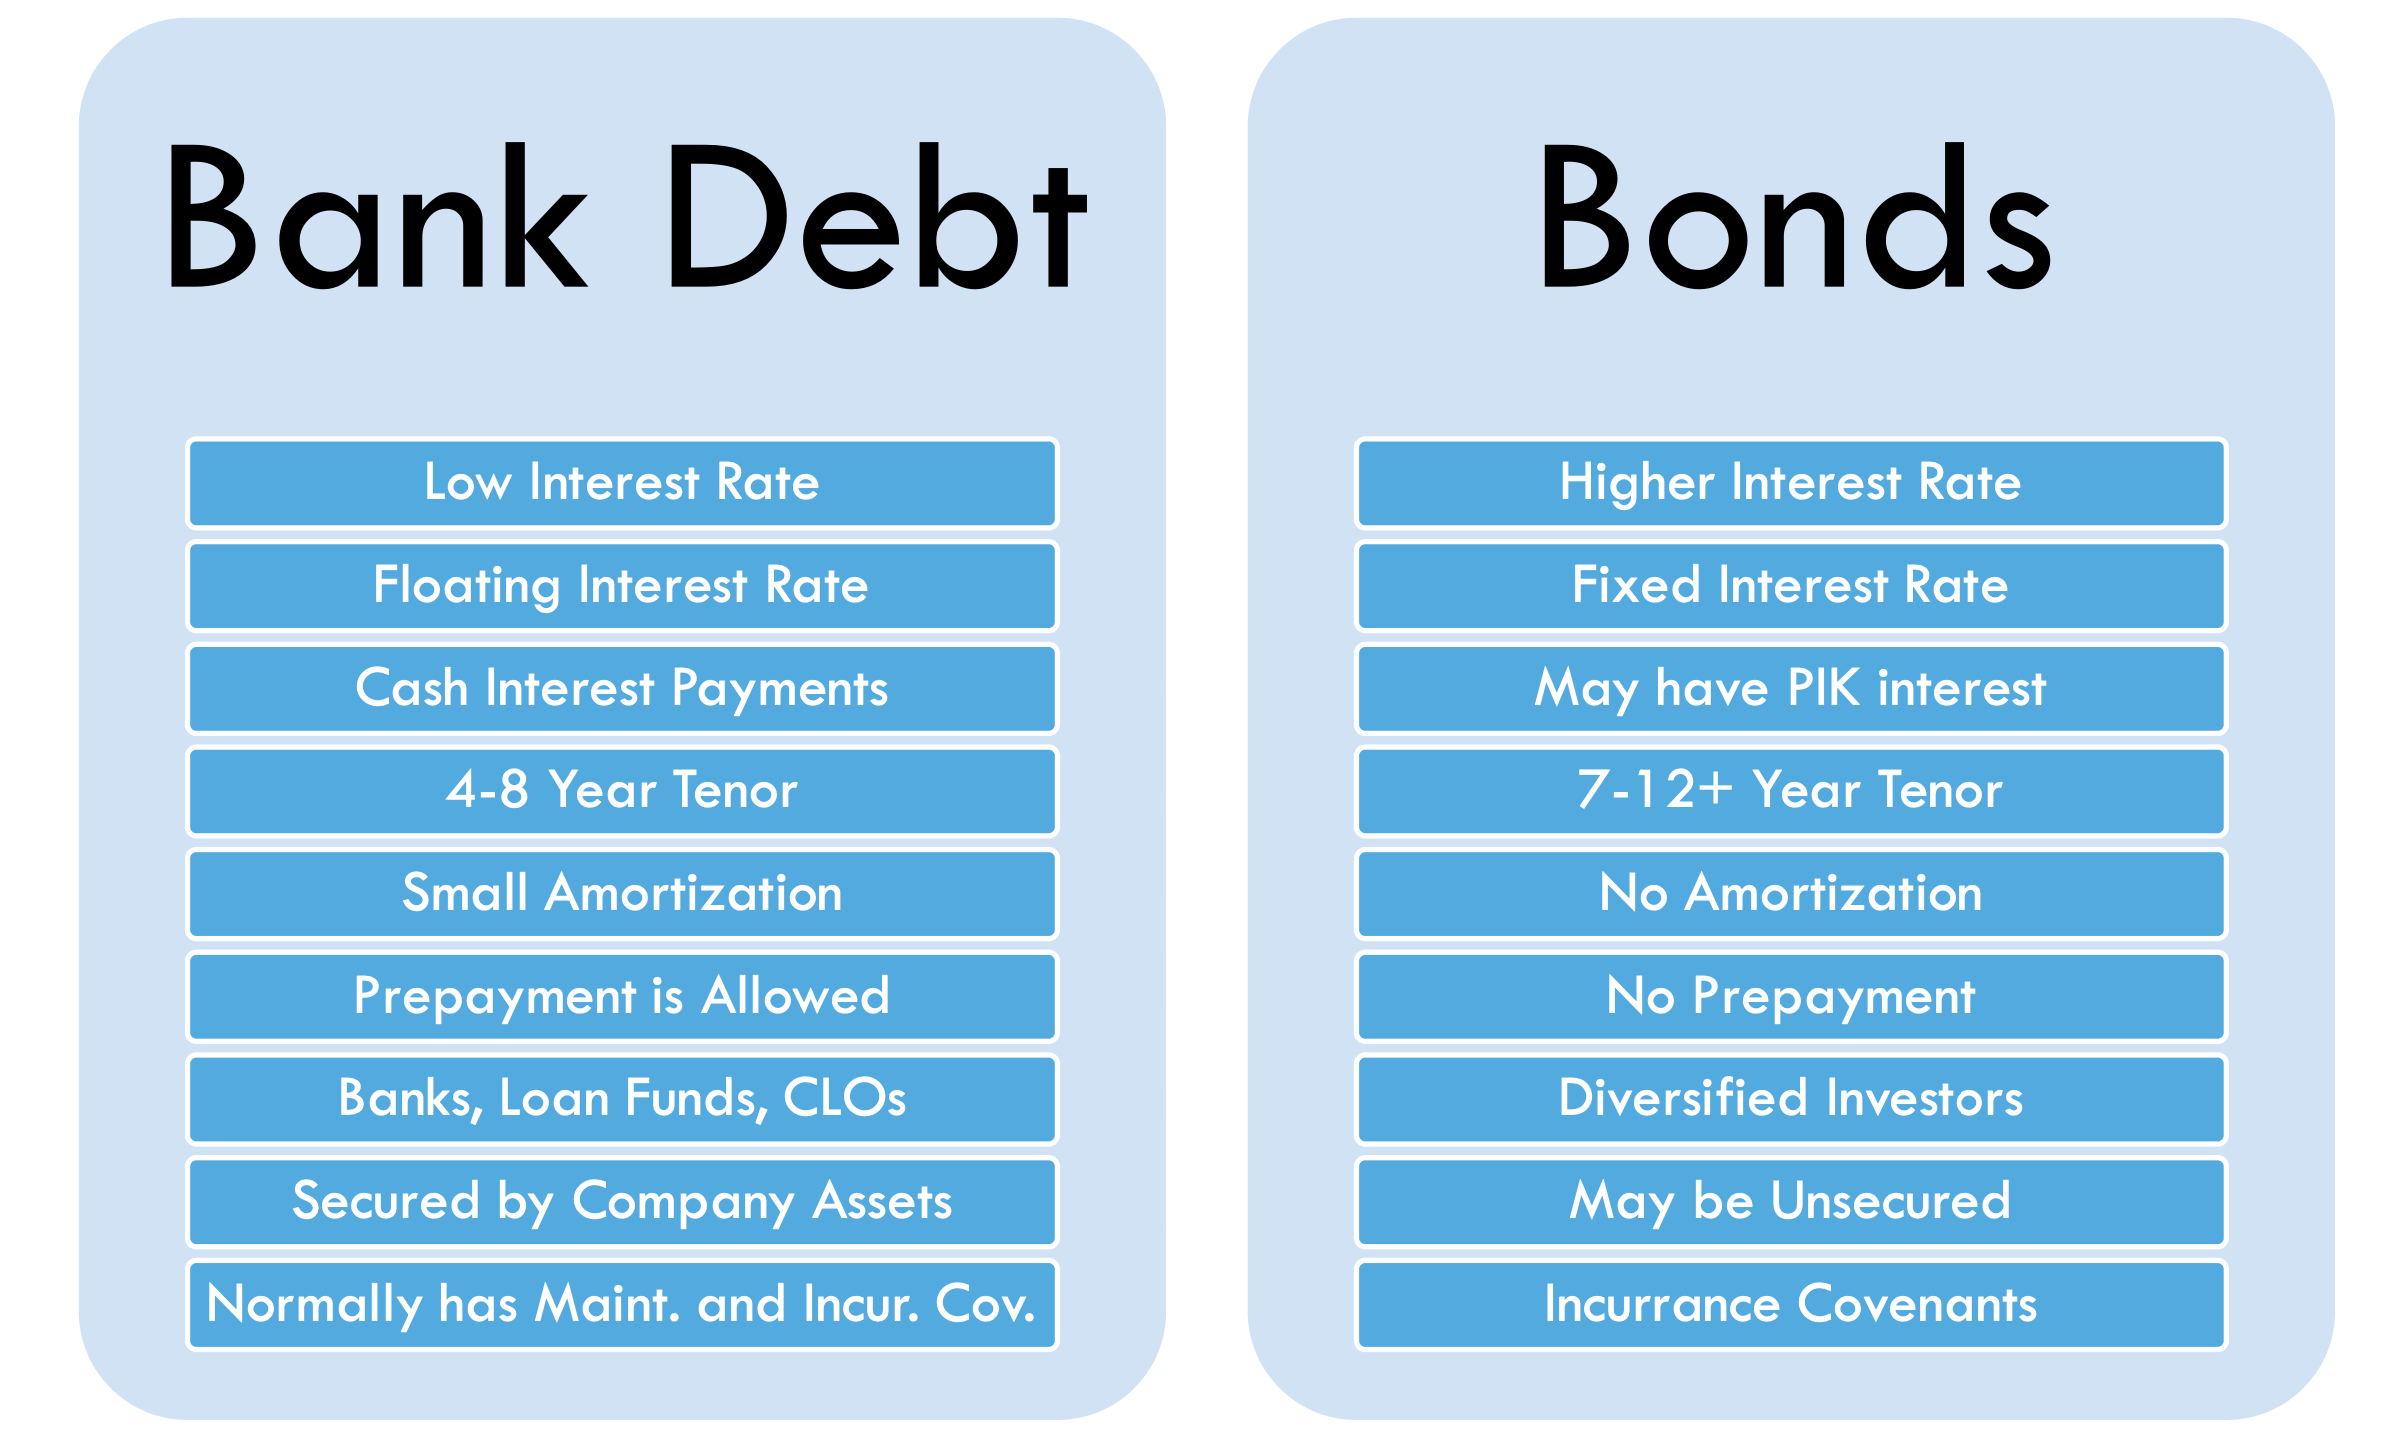
\includegraphics[width=0.5\columnwidth]{bank debt vs bond.png} % Example image
	\caption{Debt vs bond}
\end{figure}

\subsubsection{When is a bond at discount or premium ?}

If a coupon yield (coupon/face) < current yield (coupon/price) it is selling at a discount.\\
If a coupon yield of a bond > current yield then it is selling at a premium.\\

The bond price is for the secondary market.

\subsubsection{What happens if the fed raises the interest rates ?}

If the interest rate is increased the bond yield will increase, making other bonds less attractive lowering their price.

\subsubsection{What are the different types of bond ?}

\textbf{Callable bond:} Can be bought back at a premium before maturity. The issues pays back the client ending the coupon payments.\\
\textbf{Put bond:} Force the issue to buy back at face value before maturity.\\
\textbf{Convertible bond:} Bond can be converted into common stock.\\

\subsubsection{Value of perpetual bond ?}

\[ Value\:of\:PB = \frac{Coupon\:payment}{current\:interest\:rate\:on\:comparable\:bonds} \]

\subsubsection{When is debt preferred to equity ?}

\begin{itemize}
	\item Debt interest payment are tax deductible as expenses.
	\item If the stock is particularly undervalued.
\end{itemize}

\subsubsection{What is the effect of interest rate changes on bonds ?}

\begin{itemize}
	\item Zero coupon bonds will increase in price more than coupon bonds if interest rates drop.
	\item If a drop in interest rates are predicted then zero coupon bonds should be purchased.
	\item Stock markets dropping lead often lead to a switch in safer assets such as bonds.
\end{itemize}

\subsection{Credit risk analysis}

Below are a few methods to perform credit risk analysis.

\subsubsection{Current Ratio}

Current Assets / Current Liabilities

Assets should be just above liabilities for effective inventory management.

\subsubsection{Quick Ratio}

Current Assets - Inventories / Current Liabilities

More conservative than the current ratio as it assumes any inventory in the current asset cannot be easily liquidated.

\subsubsection{Interest Coverage ratio}

EBITDA / Interest Expense

Ability to make its interest payment based on earnings.

\subsubsection{Leverage Ratio}

Total Debt/EBITDA

How long before a company can retire its debt.

\subsubsection{What is a floating interest rate ?}

Used as a protection against fluctuations in interest rate.

\begin{itemize}
	\item Set by LIBOR (London interbank offer rate) plus a certain number of basis points (determined per loan)
	\item Most companies also have a LIBOR floor to prevent the rate dropping to low.
\end{itemize}

\subsubsection{What is PIK interest ?}

Paid in Kind (PIK)

\begin{itemize}
	\item Increases the face value of the bond instead of paying out coupons. This allows for compounding of value.
	\item A larger amount is paid out but only at maturity.
\end{itemize}

\subsubsection{What are covenants ?}

Legal compliance governing bonds and loans to stop defaults.

\begin{itemize}
	\item Companies breaching any covenant is technically in default.
	\item With a fee this can be waived.
\end{itemize}

\subsubsection{Revisit of Amortization}

Loan is paid off over a period of time instead of at maturity.

Reducing the face value will reduce the interest payments required.

\subsubsection{How are convertible bonds accounted for in calculating enterprise value ?}

If the conversion bond is in the money; the conversion price is below the current market price, then added as dilution to equity value. If out of the money then considered debt at face value.

\subsection{How does government influence money ?}

\begin{itemize}
	\item Buying bonds will increase the money supply.
	\item Selling bonds will decrease the money supply.
	\item Lowering interest rates will improve the money supply and vice versa.
	\item Change the banks reserve requirement
\end{itemize}

\subsubsection{What is duration ?}

How sensitive bond price is to changes in interest rates. Expressed in years.

\textbf{Formally:} The weighted average maturity of cash flows. Cash flows are the beginning of a bonds life are worth more as they have to be discounted by less years.

If cash flows faster or sooner then duration is lower and vice versa.

\subsubsection{What is convexity ?}

Convexity is the bond price vs bond yield. Higher value shows higher price and lower value shows higher payment.

The higher the convexity the more risk to fluctuations in interest rate. 

\subsubsection{What is a FICO score ?}

A credit score between 300-850

670-739 considered as good scores.

\section{Currencies}

\textbf{Spot exchange rate:} Exchange for immediate delivery. \\
\textbf{Forward exchange rate:} Exchange at some future date.

\begin{itemize}
	\item This is used by speculators to hedge exchange risk. As its an agreed set future rate will be beneficial if the prices pivot in an expected direction.
	\item The rate at which the exchange occurs can be locked in at some future date, acting as a hedge against any fluctuations.
	\item Also allows accurate budgeting and accounting.
\end{itemize}

\subsection{How is the exchange rate between two countries determined ?}

\begin{itemize}
	\item Comparing interest rates between the two countries
	\item Compare inflation
	\item Compare market cap and trading volume
\end{itemize}

\subsubsection{What is difference between currency devaluation and depreciation ?}

\textbf{Devaluation:} Controlled by the government.\\
\textbf{Depreciation:} Effected by movement in the market.

\section{Options and Derivatives}

\textbf{Derivative:} Derives its value from other asset like stocks, bonds, commodity price or market index values.\\
\textbf{Call options:} Gives the holder the right to purchase an asset for a specified exercise price on or before a specified expiration date. CALL THE CHOSEN SET PRICE.\\

if the value of the option drops below the exercise price the option is worthless as it would be cheaper to purchase from the market. \\

\textbf{Put option:} Gives the holder the right to sell an asset for a specified exercise price on or before a specified expiration date. \\

If price is above the specified sell price the option is worthless as there is more money earnt in the general market.\\

\textbf{Hedging:} Mitigate risks on an investment. \\

Invest in derivative products that have a negative correlation to the current portfolio.
Lower upside potential but provides downside protection.

\textbf{Forward contracts:} Future delivery of an asset at an agreed price. Hedge against fluctuation in the market.\\

\textbf{Future contracts:} Same as forward contracts but with strictly defined quantities of certain products traded publicly.\\

Future contracts are standardized unlike forward which are negotiated per context.

More volatile options are perceived as more valuable.

The \textbf{Black scholes model} is used to value options.

\subsection{What does an option being in the money mean ?}

\begin{itemize}
	\item Exercising the option will result in profits
	\item Call option is < the current market. Buying at lower price than the market.
	\item Put option is > the current market. Selling at higher price than the market.
\end{itemize}

\subsection{What are swaps ?}

\textbf{Swaps:} Exchange future cash flows for a period of time.\\

Conceptually one company is long on an asset with payouts along the way and another is short on an asset. An example being based on a principal amount one company will pay a fixed amount the other company will pay an amount based on the current interest rate.

\textbf{Credit default swaps:} Insurance against companies not paying their debt.\\

In a default event whatever the default swap is against the seller of the CDS will have to pay the principal amount of the asset to the CDS buyer. Until then the buyer pays a premium.

This is an effective hedge against perceived high risk assets.

\subsection{What are some metrics used in trading markets ?}

\subsubsection{Alpha}

The risk adjusted performance of an investment. Extra return above the return expected for the risk of the investment. 

\begin{table}[h] % [h] forces the table to be output where it is defined in the code (it suppresses floating)
	\centering % Centre the table
	\begin{tabular}{l l}
		\toprule
		\textbf{Metric} & \textbf{Description} \\
		\midrule
		Alpha > 0 & Returned more than expected for its level of risk.\\
		Alpha = 0 & Investment has returned the appropriate amount for its level of risk.\\
		Alpha < 0 & Investment has returned less than expected. \\
		\bottomrule
	\end{tabular}
	\caption{Alpha}
\end{table}

\subsubsection{Beta}

The volatility of the investment.

\begin{table}[h] % [h] forces the table to be output where it is defined in the code (it suppresses floating)
	\centering % Centre the table
	\begin{tabular}{l l}
		\toprule
		\textbf{Metric} & \textbf{Description} \\
		\midrule
		Beta = 1.5 & If the market rises 10\%, the investment should rise 15\% \\
		Beta = 0 & The market moves independent of the investment \\
		Beta = -1 & If the market rises 10\% the investment should fall 10\%\\ 
		\bottomrule
	\end{tabular}
	\caption{Sausage nutrition.}
\end{table}

\subsubsection{Delta}

The relationship between the price of an option and the price of the underlying security. A multiplier for the change in stock effect on option price.\\

Delta = 0.5 If the stock raises by 1 then the option price raises by 0.5 

\subsubsection{Gamma}

First derivative of delta, gauge price of option relative to how well its performing (how far in or out of the money it is.)\\

High gamma shows high risk as the price of options are rapidly changing.

\subsubsection{Rho}

Sensitivity of a derivative price in relation to fluctuations in the risk free interest rate.\\

\% Multiplier for point increases in interest rate.

\subsubsection{Theta}

How quickly a derivatives price will decline with the passage of time as the instrument approaches its exercise date. (Time decay).

\subsubsection{Vega}

How much a derivative will move with a 1\% change in volatility of the market. \\

Essentially the volatility value effects perception and therefore price.\\

Vega is high shows high volatility is causing significant change in the price. Generally positive as volatility is a positive factor for derivatives.

\section{Mergers and acquisitions}

\subsection{Why merge ?}

\begin{itemize}
	\item Synergies created by combining their operations.
	\item Example synergies: Diversify product, brand recognition, size growth, taxation (gain tax assets), management ego.
	\item A merge can also be a significant marketing ploy.
	\item Synergies should be based around EPS !
\end{itemize}

\subsection{What is the banks role in a sell side M\&A ?}

Market a company to potential buyers, then help negotiate the deal, complete and announce the sale.

\begin{enumerate}
	\item Create marketing material for the company being sold
	\item Gauge interest from potential buyers
	\item Refine buyer options
	\item Maximize deal with the chosen list of buyers 
\end{enumerate}

\subsection{What is a buy side M\&A ?}

Find potential companies for your client to acquire and negotiate a deal.

\begin{enumerate}
	\item Find acquisition targets
	\item Share with client and refine list
	\item Determine offer price
	\item Close and announce deal
\end{enumerate}

\subsection{What is the difference between strategic and financial buyer ?}

\textbf{Strategic buyer:} Acquires for strategic business reasons ie claim assets, market growth etc.\\
\textbf{Financial buyer:} Only a financial investor purchased as an asset to make profit.\\

Strategic buyers pay a premium compared to financial as they gaining more benefits than solely financial.

\subsection{What is a fairness opinion ?}

A report evaluating the facts of a M\&A transaction, examines the fairness of a given transaction.

\subsection{What is a stock swap ?}

Acquired company is paid in stock of the purchasing company. Often done when the acquired companies believes in the merge and the company has good performing stocks. 

\subsection{What is the diff between shares outstanding and fully diluted shares ?}

\textbf{Shares outstanding:}  Number of common stock issued.\\
\textbf{Fully diluted shares:} Includes all call options in the money if exercised.

\subsection{Treasury stock method}

Number of outstanding shares + options in the money exercised - the money received from the exercised options used to repurchase stocks by the company.

\subsubsection{Can you purchase a company at stock price ?}

Majority ownership comes with a control premium so the market price is not indicative.

\subsection{Should the acquire be in stock or cash ?}

Cash has taxes but is more stable and liquid. 

\subsection{What is a tender offer ?}

Acquirer offers to the purchase the stocks holders stock at higher than market price to gain controlling majority.

Can be hostile if a takeover is refused, the company instead takes control via purchasing shares (man like elon vs bird)

\subsubsection{What is divestiture ?}

A company is selling only a portion of its business not the entire company.

\subsection{What are accretive and dilutive mergers ?}

\begin{itemize}
	\item If the earnings per share EPS increase after merge then it is accretive.
	\item If the EPS decreases it is dilutive. Lost value per share during merge.
\end{itemize}

Or can use price/earning (P/E):\\

If Company Acquire P/E > Company B merge is accretive and vice versa. As the earning per share is received at a better price than the buying company has.

\subsection{Merger model basics}

Use treasury stock method which calculates the number of fully diluted shares outstanding.

Example: 1000 shares issued at market price of 5/share, 100 options issued at 2/share.

\[ Market\:cap\:(EV) = (1000 + 100 - (200/5)*5 = 1060\:shares *5 = 5300 \]

\subsection{Why is increased leverage good ?}

Increased leverage means increased returns as less of the staked money is yours, however increases financial risk.

\subsection{What do leveraged buyouts (LBO) value ?}

LBOs need cash flow to pay the debt interest payments, so steady cash flow is highly valued and generally low risk assets are chosen. 

\subsection{Why would a PE choose a risky LBO ?}

As a risky LBO with defaulting companies allow for negotiating a very good price, with a capital restructuring can lead to an sizeable return.

\subsection{What is dividend capitalization ?}

After a period of time, perhaps halfway through a LBO. New debt is collected and used to pay off the previous debt and make earnings for the owners/investors. 

\subsection{Why is an LBO a tax shield ?}

As interest payments on debt are tax deductible.

\subsection{What is Deferred tax assets (DTA) and deferred tax liabilities (DTL)?}

If an asset is written up it will have a higher depreciation short term meaning lower taxes, these taxes are recorded to be paid later as a DTL.

If an asset is written down it will have a lower depreciation short meaning higher taxes, this extra taxes are recorded as DTA.

\subsection{How to determine leverage amount ?}

A often used metric is Debt/EBITDA or leverage.

\subsection{What are the three types of merger ?}

\textbf{Horizontal merger:} Merge with competitor as a strategic business move.\\
\textbf{Vertical merger:} Supplier or distributer merge allowing cost cutting.\\
\textbf{Conglomerative merger:} Unlinked market for diversification or expansion.

\subsection{What is exchange ratio ?}

If the M\&A is funded partially or fully by stock, the stocks can be traded at a quoted exchange ratio.

This will hedge against immediate impact on the stock price after announcement, however is not as liquid.

\subsection{How can you safeguard against hostile takeover ?}

\textbf{Poison pill:} Current shareholders have the right to purchase more shares diluting the acquirers shares. Making it a less attractive purchase.\\
\textbf{Pacman:} Company being taken over reverses the situation and takes over the acquirer.\\
\textbf{White knight:} New company offers agreed friendly takeover.

\subsection{Which synergies hold more weight ?}

Cost saving synergies hold more weight due to their more immediate impact.

\section{Other}

\textbf{Institutional investor:} Pools money from other investors or clients to invest ie IB, insurance companies, pension funds etc.

\subsection{What is a Venture Capital ?}

VC are a type PE focused on high growth high risk tech companies. Many investments fail, however only need a few to be a success.

\subsection{What are Hedge funds ?}

\begin{itemize}
	\item Loosely regulated investment pool
	\item Limited to high net individuals (100-500 investor cap)
	\item Hedge against risk to make profits often use high leverage with high risk for sizable returns
\end{itemize}

\subsection{What is securitization ?}

Bundle together group of assets to be create a new financial investment tool. Staged in different tiers called tranches.

\subsection{What is arbitrage ?}

Buying and selling two related assets to gain guaranteed profits due to inaccurate market prices.

%----------------------------------------------------------------------------------------
%	FIGURE EXAMPLE
%----------------------------------------------------------------------------------------

% \begin{figure}[h] % [h] forces the figure to be output where it is defined in the code (it suppresses floating)
% 	\centering
% 	\includegraphics[width=0.5\columnwidth]{IMAGE_NAME.jpg} % Example image
% 	\caption{European swallow.}
% \end{figure}

%----------------------------------------------------------------------------------------
% MATH EXAMPLES
%----------------------------------------------------------------------------------------

% \begin{align} 
% 	\label{eq:bayes}
% 	\begin{split}
% 		P(A|B) = \frac{P(B|A)P(A)}{P(B)}
% 	\end{split}					
% \end{align}

%----------------------------------------------------------------------------------------
%	LIST EXAMPLES
%----------------------------------------------------------------------------------------

% \begin{itemize}
% 	\item First item in a list 
% 		\begin{itemize}
% 		\item First item in a list 
% 			\begin{itemize}
% 			\item First item in a list 
% 			\item Second item in a list 
% 			\end{itemize}
% 		\item Second item in a list 
% 		\end{itemize}
% 	\item Second item in a list 
% \end{itemize}

%------------------------------------------------

% \subsection{Numbered List}

% \begin{enumerate}
% 	\item First item in a list 
% 	\item Second item in a list 
% 	\item Third item in a list
% \end{enumerate}

%----------------------------------------------------------------------------------------
%	TABLE EXAMPLE
%----------------------------------------------------------------------------------------

% \section{Interpreting a Table}

% \begin{table}[h] % [h] forces the table to be output where it is defined in the code (it suppresses floating)
% 	\centering % Centre the table
% 	\begin{tabular}{l l l}
% 		\toprule
% 		\textit{Per 50g} & \textbf{Pork} & \textbf{Soy} \\
% 		\midrule
% 		Energy & 760kJ & 538kJ\\
% 		Protein & 7.0g & 9.3g\\
% 		\bottomrule
% 	\end{tabular}
% 	\caption{Sausage nutrition.}
% \end{table}

%----------------------------------------------------------------------------------------
%	CODE LISTING EXAMPLE
%----------------------------------------------------------------------------------------

% \begin{lstlisting}[
% 	caption= Macro definition, % Caption above the listing
% 	language=python, % Use Julia functions/syntax highlighting
% 	frame=single, % Frame around the code listing
% 	showstringspaces=false, % Don't put marks in string spaces
% 	numbers=left, % Line numbers on left
% 	numberstyle=\large, % Line numbers styling
% 	]

% 	CODE

% \end{lstlisting}

%----------------------------------------------------------------------------------------
%	CODE LISTING FILE EXAMPLE
%----------------------------------------------------------------------------------------

% \lstinputlisting[
% 	caption=Luftballons Perl Script., % Caption above the listing
% 	label=lst:luftballons, % Label for referencing this listing
% 	language=Perl, % Use Perl functions/syntax highlighting
% 	frame=single, % Frame around the code listing
% 	showstringspaces=false, % Don't put marks in string spaces
% 	numbers=left, % Line numbers on left
% 	numberstyle=\tiny, % Line numbers styling
% 	]{luftballons.pl}

%------------------------------------------------

\end{document}